\subsection{Brechzahlprofile}
\label{subsec:pofbrechzahlprofile}

Um die Bandbreite von einem POF-Kabel zu erhöhen kommen Faser zum Einsatz deren
Brechzahlen modifiziert wurden.

\subsubsection{Stufenindexprofil (SI-POF)}

Der Stufenindex ist durchsatzschwächste Brechzahlprofil (ca. 100 Megabit/s auf
100 m, spezielle Übertragungsverfahren erlauben Bitraten im Bereich von 1
Gigabit/s). Als Kernmaterial wird Polymethylmethacrylat mit einem Durchmesser
von ca. 1 mm, welcher von einem ca. 10 µm Mantel umgeben ist, eingesetzt
\cite{pofacsi}. \autoref{fig:pofsi} fasst den Aufbau und die Lichtausbreitung
zusammen. Die Spalte mit Brechungsindex als Überschrift stellt den Verlauf
dieses grafisch dar. Beim Stufenindexprofil steigen die Brechzahlen beim
Übergang vom Mantel zum Kern abrupt an. Dies hat die schon erwähnte
Totalreflexion an der Kerngrenze, welche man in der Spalte Querschnitt erkennen
kann, zur Folge.

\begin{figure}[h]
    \begin{center}
        \begin{minipage}[t]{0.4\textwidth}
            \begin{center}
                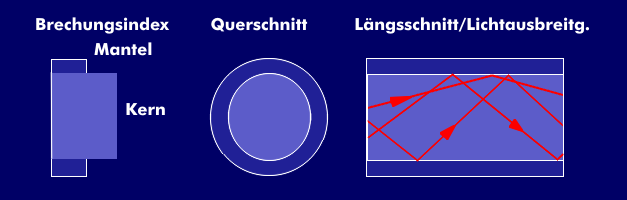
\includegraphics[width=0.9\textwidth]{Bilder/Optische_Wellenleiter_Die_Polymer_Optische_Faser/Brechzahlprofile/pofsi.png}
                \caption[Aufbau des Stufenindexprofils \newline \url{http://www.itwissen.info/bilder/aufbau-und-brechungsprofil-der-stufenindex-profilfaser.png} (zuletzt aufgerufen am 19.09.2015)]{Aufbau des Stufenindexprofils}
                \label{fig:pofsi}
            \end{center}
        \end{minipage}
        \hspace{0.025\textwidth}
        \begin{minipage}[t]{0.4\textwidth}
            \begin{center}
                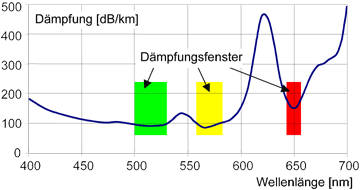
\includegraphics[height=0.1\textheight]{Bilder/Optische_Wellenleiter_Die_Polymer_Optische_Faser/Funktionsweise/pofdaempfung.png}
                \caption[Dämpfungsfenster bei einer polymer optischen Faser \newline \url{http://www.pofac.fh-nuernberg.de/pofac/de/was_sind_pof/images/pmma_daempfung.png} (zuletzt aufgerufen am 19.09.2015)]{Dämpfungsfenster beim Stufenprofil}
                \label{fig:pofdaempfung}
            \end{center}
        \end{minipage}
    \end{center}
\end{figure}

\autoref{fig:pofdaempfung} zeigt die Dämpfungsfenster einer polymer optischen
Faser. Diese liegen bei den Farben grün, gelb und rot. Um die Intensitätsabnahme
möglichst gering zu halten und damit die Reichweite zu erhöhen werden
Wellenlängen für die Lichtimpulse gewählt, die in den Dämpfungsfenstern liegen.
Als Lichtquelle kann zum Beispiel eine LED verwendet werden und als Empfänger
kommen Photodetektoren zum Einsatz. Der geringe Preis und die robuste
Übertragung auf kurzen Strecken machen die SI-POF zu einer beliebten alternative
gegenüber von Kupferkabeln in Industrieanlagen oder in Fahrzeugen. \cite{poflee}

\subsubsection{Gradientenindexprofil (GI-POF)}

Das Gradientenindexprofil bittet mit bis zu 40 Gigabit/s auf 100m deutlich
höhere Bitraten als das Stufenindexprofil. Beim Gradientenindex nimmt der
Brechungsindex vom Mantel bis zur Mitte des Kern kontinuierlich zu (siehe
\autoref{fig:pofgi} Spalte Brechungsindex). \autoref{fig:pofgi} zeigt ebenfalls
in der Spalte Längsschnitt den daraus resultierenden Lichtstrahlenverlauf.
Dieser verläuft, im Gegensatz zu der geraden Lichtausbreitung beim Stufenindex,
sinusförmig. Der Kerndurchmesser der GI-POF ist mit ca. 100 µm um das 10fache
geringer als der einer SI-POF. Dadurch werden geringere Laufzeitunterschiede
ermöglicht und die Frequenz der Lichtimpulse kann erhöht werden. Außerdem wird
bei der GI-POF eine Dämpfung von unter 20 dB/km erreicht. Dies ist eine
ehrheblicher Verbesserung gegenüber der Dämpfung von SI-POF mit ca. 100 dB/km
(siehe \autoref{fig:pofgidaempfung}). Aus den beiden Gründen ist die Bandbreite
einer Faser mit Gradientenindex significant höher als die einer einer Faser mit
Stufenindex. Als Kernmaterial kann hier der Kunststoff
CYTOP\textsuperscript{\texttrademark} der Asahi Glass Co., Ltd. oder
Polymethylmethacrylat verwendet werden \cite{pofacgif}. Aufgrund der hohen
Bitraten und der Biegsamkeit werden GI-POF in \shorthandoff{"}"Local Area
Networks"\shorthandon{"} (LAN) und in Supercomputern eingesetzt \cite{poflee}.

\begin{figure}[h]
    \begin{center}
        \begin{minipage}[t]{0.4\textwidth}
            \begin{center}
                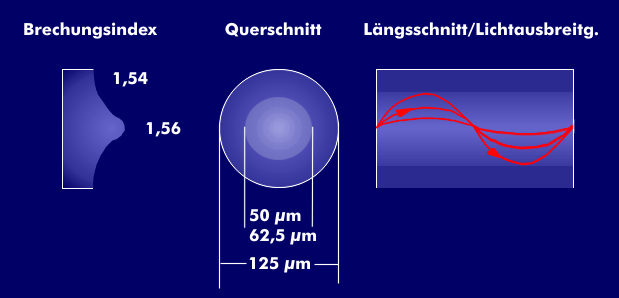
\includegraphics[width=0.9\textwidth]{Bilder/Optische_Wellenleiter_Die_Polymer_Optische_Faser/Brechzahlprofile/pofgi.png}
                \caption[Aufbau des Gradientenindexprofils \newline \url{http://www.itwissen.info/bilder/aufbau-und-brechungsprofil-der-gradientenfaser.png} (zuletzt aufgerufen am 19.09.2015)]{Aufbau des Gradientenindexprofils}
                \label{fig:pofgi}
            \end{center}
        \end{minipage}
        \hspace{0.025\textwidth}
        \begin{minipage}[t]{0.4\textwidth}
            \begin{center}
                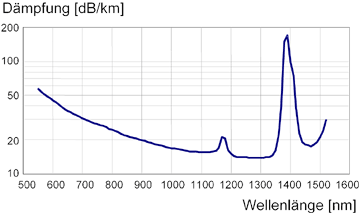
\includegraphics[height=0.1\textheight]{Bilder/Optische_Wellenleiter_Die_Polymer_Optische_Faser/Brechzahlprofile/pofgidaempfung.png}
                \caption[Dämpfung bei einer GI-POF \newline \url{http://www.pofac.fh-nuernberg.de/pofac/de/was_sind_pof/images/gradientenindex_daempfung.png} (zuletzt aufgerufen am 19.09.2015)]{Vergleich der Dämpfungswerte von GI-POF und SI-POF}
                \label{fig:pofgidaempfung}
            \end{center}
        \end{minipage}
    \end{center}
\end{figure}


\subsubsection{Weitere Profile}

Weitere Erhöhungen der Bandbreite werden durch mehrere Mäntel (siehe
\autoref{fig:pofdsi} \autoref{fig:pofmsi}, Reduzierung der Laufzeitunterschiede)
bzw. durch mehrere Kerne (siehe \autoref{fig:pofmc}, mehrere Lichtstrahlen
gleichzeitig) innerhalb eines Kabels erreicht. \autoref{fig:pofdsimc} zeigt eine
Kombination der beiden obigen Optimierungsmöglichkeiten.
\cite{pofacprofile}

\begin{figure}[h]
    \begin{center}
        \begin{minipage}[t]{0.4\textwidth}
            \begin{center}
                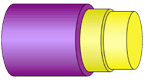
\includegraphics[height=0.1\textheight]{Bilder/Optische_Wellenleiter_Die_Polymer_Optische_Faser/Brechzahlprofile/pofdsi.png}
                \caption[\shorthandoff{"}"\shorthandon{"}\shorthandoff{"}Dual
                Step Index"\shorthandon{"} - POF (zwei Mäntel, Stufenindex)
                \newline
                \url{http://www.pofac.fh-nuernberg.de/pofac/de/was_sind_pof/images/profil_dsi-pof.png} (zuletzt aufgerufen am 19.09.2015)]{\shorthandoff{"}"\shorthandon{"}\shorthandoff{"}Dual Step Index"\shorthandon{"} - POF (zwei Mäntel, Stufenindex)}
                \label{fig:pofdsi}
            \end{center}
        \end{minipage}
        \hspace{0.025\textwidth}
        \begin{minipage}[t]{0.4\textwidth}
            \begin{center}
                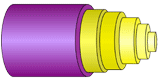
\includegraphics[height=0.1\textheight]{Bilder/Optische_Wellenleiter_Die_Polymer_Optische_Faser/Brechzahlprofile/pofmsi.png}
                \caption[\shorthandoff{"}"\shorthandon{"}\shorthandoff{"}Multi
                Step Index"\shorthandon{"} - POF (mehrere Mäntel, Stufenindex)
                \newline
                \url{http://www.pofac.fh-nuernberg.de/pofac/de/was_sind_pof/images/profil_msi-pof.png} (zuletzt aufgerufen am 19.09.2015)]{\shorthandoff{"}"\shorthandon{"}\shorthandoff{"}Multi Step Index"\shorthandon{"} - POF (mehrere Mäntel, Stufenindex)}
                \label{fig:pofmsi}
            \end{center}
        \end{minipage}
    \end{center}

    \begin{center}
        \begin{minipage}[t]{0.4\textwidth}
            \begin{center}
                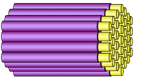
\includegraphics[height=0.1\textheight]{Bilder/Optische_Wellenleiter_Die_Polymer_Optische_Faser/Brechzahlprofile/pofmc.png}
                \caption[\shorthandoff{"}"\shorthandon{"}\shorthandoff{"}Multi
                Core"\shorthandon{"} - POF (mehrere Kerne, Stufenindex) \newline
                \url{http://www.pofac.fh-nuernberg.de/pofac/de/was_sind_pof/images/profil_mc-pof.png} (zuletzt aufgerufen am 19.09.2015)]{\shorthandoff{"}"\shorthandon{"}\shorthandoff{"}Multi Core"\shorthandon{"} - POF (mehrere Kerne, Stufenindex)}
                \label{fig:pofmc}
            \end{center}
        \end{minipage}
        \hspace{0.025\textwidth}
        \begin{minipage}[t]{0.4\textwidth}
            \begin{center}
                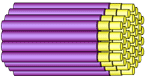
\includegraphics[height=0.1\textheight]{Bilder/Optische_Wellenleiter_Die_Polymer_Optische_Faser/Brechzahlprofile/pofdsimc.png}
                \caption[\shorthandoff{"}"\shorthandon{"}\shorthandoff{"}Dual
                Step Index - Multi Core"\shorthandon{"} - POF (mehrere Kerne,
                zwei Mäntel, Stufenindex) \newline
                \url{http://www.pofac.fh-nuernberg.de/pofac/de/was_sind_pof/images/profil_dsi-mc-pof.png} (zuletzt aufgerufen am 19.09.2015)]{\shorthandoff{"}"\shorthandon{"}\shorthandoff{"}Dual Step Index - Multi Core"\shorthandon{"} - POF (mehrere Kerne, zwei Mäntel, Stufenindex)}
                \label{fig:pofdsimc}
            \end{center}
        \end{minipage}
    \end{center}
\end{figure}
